%%%%%%%%%%%%%%%%%%%%%%%%%%%%% BEGIN PACKAGE
\documentclass[11pt]{amsart}       % AMS template just for the draft
\usepackage{geometry}                 % See geometry.pdf to learn the layout options. There are lots.
\geometry{a4paper}                        % .letter or a4paper or a5paper or ... 
%\geometry{landscape}                 % Activate for for rotated page geometry
%\usepackage[parfill]{parskip}     % Activate to begin paragraphs with an empty line rather than an indent
\usepackage{graphicx}                   % FIgure
\usepackage{amssymb}                 % Math symbol
\usepackage{epstopdf}                   % for working in .pdf and  not .dvi (convert .eps, .jpg,  etc to .pdf)
\usepackage{psfrag}
\usepackage[T1]{fontenc}
\usepackage{aeguill}
\DeclareGraphicsRule{.tif}{png}{.png}{`convert #1 `dirname #1`/`basename #1 .tif`.png}
%%%%%%%%%%%%%%%%%%%%%%%%%%%%% END PACKAGE
\graphicspath{{PLOT/SinglePDGEMM/}{PLOT/VectorPDGEMM/}}

%%%%%%%%%%%%%%%%%%%%%%%%%%%%% BEGIN AUTHORS AND INSTITUTIONS
\title{Ambient: overview of the workflow and design basics}
\author[A. Kosenkov, T. Ewart, B. Bauerb, A. Kantian,  M. Troyer, T. Giarmarchi]{Alexandr Kosenkov, Timoth\'ee Ewart, Bela Bauer, Adrian Kantian, Matthias Troyer and Thierry Giamarchy }

%%%%%%%%%%%%%%%%%%%%%%%%%%%%% BEGIN AUTHORS AND INSTITUTIONS


%%%%%%%%%%%%%%%%%%%%%%%%%%%%% BEGIN MACRO
\makeatletter
\newcommand\etc{\textit{etc}\@ifnextchar.{}{.\@}}
\newcommand\eg{\textit{e.g. }}
\newcommand\ie{\textit{i.e. }}
\newcommand\cf{\textit{c.f. }}
\renewcommand{\labelitemi}{$\diamond$}


\makeatother
%%%%%%%%%%%%%%%%%%%%%%%%%%%%% END MACRO
\begin{document}

%%%%%%%%%%%%%%%%%%%%%%%%%%%%% BEGIN SYMBOL
\def\cloud{
\includegraphics[width=0.2cm]{FIGURES/cloud}}
%%%%%%%%%%%%%%%%%%%%%%%%%%%%% END SYMBOL
\maketitle

%%%%%%%%%%%%%%%%%%%%%%%%%%%%% BEGIN INTRODUCTION
\section{Introduction}

%Nowadays, the numerical simulations get an essential position, as experiments,  for studying physical 
%properties of many problems. The numerical simulations are presented inside every fields of sciences 
%and engineering, as classical and quantum mechanic, quantum chemistry,  \etc. As usual, the users always
%want increase the size of their problems, as billion number of particles for a kinetic simulation, billion 
%of meshes for a fluid dynamic computation, or else, matrixes of million entries for a quantum mechanic,
%or the linear algebra problems. Thus, the high performance computing is the solution for solving very large problem,
%with the peta flops  and the future generation of exa flops computers, the engineers and the scientists will
%have a quasi unlimited set of resources for modeling, nevertheless, they will be confronted to a challenge, have compatible
%programs for these machines. 

%A large set of programs; solvers, and software solutions are now availabled to solve large problem in a lot of fields, \eg we can 
%cite as popular in a few scientist field :  {\sc Quantum ESPRESSO} \cite{QE-2009} in quantum chemistry, Abinit \cite{ABINIT-2005, ABINIT-2009} in quantum mechanic,  ScaLAPACK \cite{SCALAPACK-1997} in linear 
%algebra,  or else SMILE in hypersonic rarefied flow \cite{SMILE-2005}. Of course, this short list is not exhaustive,
%and it can be fill up easily in every fields of science and engineering.

%If the scientists or the  engineers have the right tools, it will be necessarily  limited by the scalability of the code, in the case of the famous mathematical library ScaLAPACK, the
%efficiency  and thus the scalability, with the appropriated setting will reach up to 512 processors ($\sim  \mathcal{O}(100)$) \cite{SCALAPACK-1992}, beyond the interest is useless
%due to the degradation of the performance. In the worst case, the programmers will start  from a white page, and must design and efficient code.
%Due to the incredible number of cores, and optional accelerators as GPU, FGPA or "CELL like\footnote{Although the CELL processor is now depreciated, it herebies  
%a way of integrated processor (CPU+GPU), as the prove the last processor products of Intel (core i series) and AMD (fusion).}", the programmers 
%will have to introduce a mix programming model usually named mix-mode, based on a main MPI layer coupled with one or several additional layers \cite{EXASCALE-2010}.

%The most popular layer for mix-mode is OpenMP, and it is based on the preprocessor directives \texttt{\#pragma}, it demonstrated its performance. It is included successfully inside
%the  linear algebra libraries like the MKL from Intel or the PESSLSMP from IBM.  This ideology of the utilization of the pre-directives becomes more and more 
%important, thus it is used for vectorization of loops using the intel compiler and even for GPU with the PGI compiler. Although this ideology gives results, there is 
%a limitation for the main following reason: the creation/destruction of the threads will be extremely time consuming,
%when the  grain problem size becomes too fine \cite{SMITH-2001}. To achieve the best performance, the number of thread should be  equal to the number of cores on a socket, 
%thus the scalability will be increased at maximum by an order of magnitude.  The maximum number of processors now reach, becomes ($\sim \mathcal{O}(1000)$). 
%This ideology of implementation of the mix mode is more an evolution of the programming model than a revolution. It is an fast hand-on to implement that prolongates the life and the performance on a existing code. But,
%it will not prepare at all the code for the future, that will be automatically depreciated  by the new generation of cluster, in term of scalability.
   
%For getting several order of magnitude higher, we need a new programming model. The introduction of the GPU computing by NVidia a few years ago was
%a real innovation in HPC \cite{NICKOLLS-2010}. On a GPU, it is usual to program  thousand of threads. Thus, in this paper, we propose a innovative programming model to program on very large distributed cluster. We develop
%a framework named Ambient (C++) where we expend the CUDA programming ideology to  the a full cluster, thus we keep away the MPI programming model from the users.  In a way, we  extended
%the philosophy of OpenCL, OpenCL extents  the GPU programming model to a processor, assimilate a socket as a GPU, where every cores of the socket are assimilated to a streaming processor.
%We also developed inside a dynamic stack manager, that stocks and manages the execution of numerical "operations-solver" in functions of the resources of the distributed cluster.
   
%In this paper, we are going to describe our object oriented framework, and promote a first application based on linear algebra. Our main objective, is to 
%promote a new technology to develop  parallel application, without any interaction with the MPI and thread layer, and allow, a real access in term of performance to the next generation
%of clusters. The first possible  targets are applications that require large buffer of contiguous memory: quantum mechanic, linear algebra,  computational fluid dynamics, molecular dynamic \ldots 
%\, Until the end of this paper, we will focus on the linear algebra problems and their applications.


- Stress Performance of Ambient 
  - in terms of flexible and dynamical resource allocation
  - Stress performance boost derived from this (we need the benchmarks for that!)

%%%%%%%%%%%%%%%%%%%%%%%%%%%%% END INTRODUCTION


%%%%%%%%%%%%%%%%%%%%%%%%%%%%% BEGIN WORKFLOW
\section{Ambient workflow}

Before presenting various elements of Ambient in more detail, this section provides the
workflow of execution for an Ambient-parallelized application in general terms. 
As the Ambient computational architecture derives from CUDA, we start with a simplified
workflow of execution for both CUDA-enabled and Ambient enabled applications side-by-side:

\begin{table}[h]  
	\begin{center}
	 	\begin{tabular}{l l  l l} % L L  L L 
                        \hline 
                             \multicolumn{2}{c}{CUDA} &  \multicolumn{2}{c}{Ambient} \\
                             \hline
                             \multicolumn{4}{c}{  $\diamond$ Serial code}  \\
                            $\diamond$ & Kernel encountered                                  &  $\diamond$ & Kernel-pair (logistic/computa- \\
                               & & & tional) encountered \\
                               $\diamond$ &Thread block grid construction&     $\diamond$  & Kernel-pair stacked for later  \\
                                &(gridDim, blockDim)  &  &  execution  \\ 
                               $\diamond$ &  Thread blocks mapping onto de-  &  &  \\
                                & vice (GPU SMPs) &  & \\
                               $\diamond$ &  Execution of kernel: GPU SMP & & \\
                               &  executes kernel on every thread& &    \\
                               &  of corresponding thread blocks  & & \\
                               \multicolumn{4}{c}{  $\diamond$ Serial code}  \\
                               & &    $\diamond$&Stack flush signal encountered : \\
                               & & & execution of kernels \\
                                  \hline
        		 \end{tabular}  
              \caption{Workflow analogy between the execution of a CUDA and a Ambient application} \label{WORKFLOW}
	\end{center}
\end{table}

As soon as Ambient encounters the flush signal [MORE EXPLANATION]- kernel
execution is initiated along the following sequence:

\begin{itemize}
\item Execution of logistic kernel: allocation of device (MPI group) according to specified request. 
\item Execution of logistic kernel: argument's work groups decomposition according to workDim [MORE EXPLANATION].
\item Execution of logistic kernel: selected argument's work groups mapping onto device (MPI processes). [MORE EXPLANATION]
\item Transfer of work groups to the target processes.
\item Execution of computational kernel: MPI process executes kernel thread for work items of assigned work groups.
\end{itemize}

The main reason for the difference in workflow compared to CUDA is the scale of available resources.  As practically unlimited resources
are available for a kernel's launch, the data becomes the key factor around which Ambient's design evolves.
In particular, in order to control the data movements and resource usage, we introduce the logistic kernel and make kernel calls non-blocking. 

Generally, Ambient enabled applications operate with abstract types that already have tiled memory structure. Upon encountering a kernel operation 
call, the Ambient framework stacks the operation for later execution and proceeds in this manner through the serial code. This design
enables a high degree of reusage of the original serial code, while providing powerful instrumentation capabilities to manage resources and tune performance 
of the application overall.

When the framework encounters the signal to flush the stack of kernels the actual execution starts. The framework's engine goes through the accumulated stack 
and executes all independent operations at once. Executing an operation, the engine first invokes the associated logistic kernel and allocates a specified
amount of resources for this operation. Next, the engine sets the argument's (here: the matrices) tiling using user specified work group sizes and maps resulting work groups onto allocated
processes. Now the engine can freely transfer the tiled data from previous owners to the allocated processes changing
the tile size if needed. After the transfer is complete the computational kernel kicks in behaving almost the same way as in CUDA, with work groups
simply being mapped onto threads of MPI process as if they were GPU SMP (the difference lies mainly in the user's control over the mapping of processes to work groups).

In the following sections, we elaborate on the role and functionalities of the different elements listed here.

%%%%%%%%%%%%%%%%%%%%%%%%%%%%% END WORKFLOW


%%%%%%%%%%%%%%%%%%%%%%%%%%%%% BEGIN DESCRIPTION OF THE FRAMEWORK
\section{Design of the framework}
%In this section, we describe our framework in simple terms, without  a deep technical description.
%We will focus on the main functionalities  and show the essential features.

%%%%%%%%%%%%%%%%%%%%%%%%%%%%% BEGIN CUDA IDEOLOGY SECTION
\subsection{Extending the CUDA approach} \label{CUDAIDEOLOGYSECTION}

Ambient employs an extension of the CUDA approach onto a distributed cluster. This is based on the observation that modern clusters employ many thousands of nodes, just like a GPU consists of thousands of small, simple cores, on each of which it runs an independent thread. In such a comparison however, the technical specifics of the basic cluster unit in terms of processor power, memory bandwidth, network speed, \etc  \, must be considered. 

A CPU core has much higher capabilities than a GPU core, and thus we can't simply downcast the CPU core to the GPU one.
Therefore, the scope of the data for a single CPU (on which a single Ambient thread typically runs) in Ambient is rather comparable to the capacity of CUDA's thread block or an OpenCL work group. The typical block size is $ 128 \times 128$, although, the user has full control of this size and can adapt it to the needs of the target problem. As in CUDA, work groups and corresponding grid of groups are formed in Ambient. A basic comparison between CUDA and Ambient is shown in table \ref{ANALOGY}.

\begin{figure}[t]
	\begin{center}
	                  %psfrag for changing the layout
	                  \psfrag{New data layout}{\tiny{new layout}}
			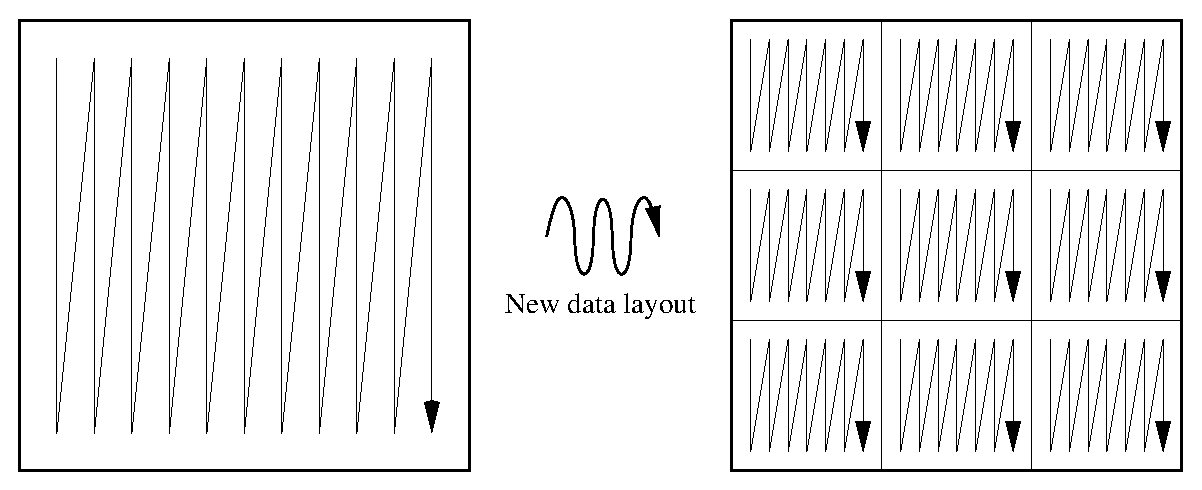
\includegraphics[scale=0.44]{FIGURES/MemMatrix.eps} 
	\end{center}
          \caption{Representation of the data layout inside the memory. Instead of the single contiguos block's layout we use tiled layout.}
          \label{MEMMATRIX}
\end{figure}

The work group approach imposes the data layout of the framework. The standard math libraries impose both column order as well as a contiguous memory order on a matrix storage (figure \ref{MEMMATRIX}).

Therefore, we keep the column order but do not conserve a full contiguous buffer. As in the PLASMA library \cite{LTAIEF-2011}, we choose
a tile data layout. It allows to avoid penalties due to NUMA nature of memory allocation on the CPU (section \ref{MPIABSTRACTION}) and, naturally, this data layout supports the work group representation of execution, as shown in Fig. \ref{CUDAANALOGY}. 

In CUDA and OpenCL, the execution model imposes kernel initialization with the appropriate resources (\eg block and grid dimensions),
after which the user does not have to explicitely manage the memory transfer inside the GPU; due to the distributed memory of clusters and the frequently heterogeneous nature of processing units we need both fine-grained control of the work group per process assignement as well as of the memory transfer operations. That should be done in a simple, automatic yet flexible way. In order to achieve this goal we split the kernel invocation into two parts.

First, we prepare the memory of corresponding work groups. Then we execute our numerical operations \eg a matrix multiplication in the following sequence \footnote{From here onwards, we will illustrate the execution model through parallel matrix addition or multiplication.}:
\begin{enumerate}
	\item A logistic kernel; where we select the number of processors, and map the data onto processes indices (???).
	\item A computational kernel; where we execute required computational operations (similar to the CUDA-kernel).
\end{enumerate}

Thus, every operation (\eg multiplication, addition, or more sophisticated linear algebra operations) will have an associated logistic and computational kernel. 

\newpage

\begin{figure}[!t]
	\begin{center}
           	        \psfrag{Ambient representation}{\tiny{\hspace{-0.4cm}Ambient representation}}
           	        \psfrag{CUDA/OpenCL representation}{\tiny{\hspace{-0.9cm}CUDA/OpenCL representation}}
	                 \psfrag{Associated mapping of the data with Ambient}{\tiny{\hspace{+0.15cm}Associated data mapping}}
	                 \psfrag{1x1 workgroup}{\tiny{\hspace{-0.5cm} \vspace{-0.1cm}1x1 workgroup}}
	                  \psfrag{of Ambient}{\tiny{\hspace{-0.4cm}\vspace{-0.9cm} of Ambient}}
	                  \psfrag{Workgroup of 4X4 threads}{\tiny{\hspace{-0.5cm} \vspace{-0.1cm}4x4 workgroup}}
	                  \psfrag{of CUDA}{\tiny{\hspace{-0.25cm}of CUDA}}
	                  \psfrag{Scope of GPU thread (left)}{\tiny{\hspace{-0.25cm}GPU scope left}}
	                  \psfrag{CPU (right)}{\tiny{\hspace{-0.7cm}CPU scope right}}       
		        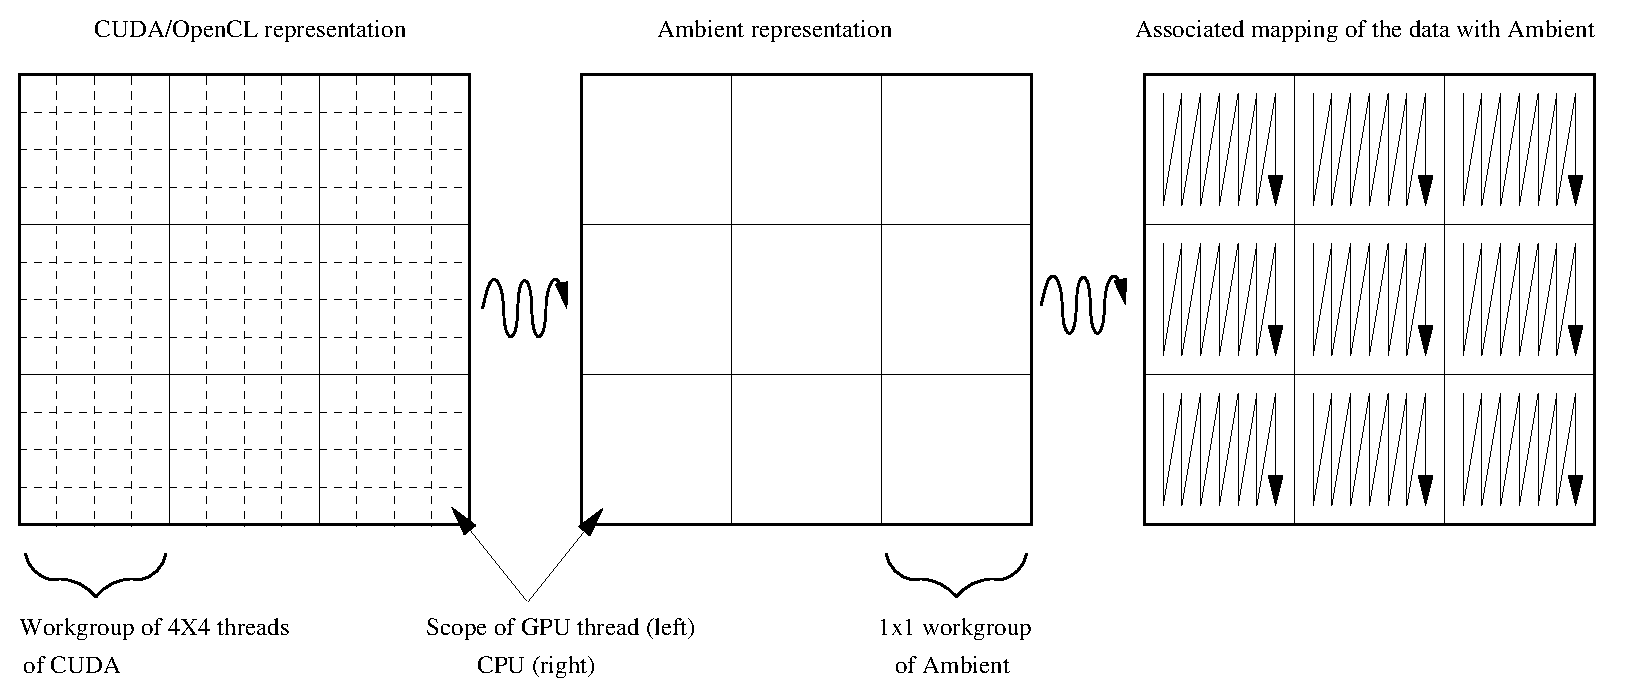
\includegraphics[scale=0.44]{FIGURES/CUDAanalogy.eps} 
	\end{center}
          \caption{Similarity between CUDA's thread grid and Ambient's work group grid (with tiles mapped to work groups).}
          \label{CUDAANALOGY}
\end{figure}
\begin{table}[h]
	\begin{center}
	 	\begin{tabular}{c  c  c}
		 	                                                      & CUDA/OpenCL                                & Ambient            \\  \hline 
			 Device                                        & GPU or CPU (socket)   & Cluster               \\  
			  Entity  of Calculation               & GPU-Thread                                      & CPU-Thread     \\  
			 \begin{tabular}{c}
			 Scope of the \\ 
			 entity calculation  
                             \end{tabular}
                             &  Buffer entry                            & Full buffer \\
			 Execution model                       & Kernel                                                &  \begin{tabular}{c}  Logistic and \\ computational kernel   \end{tabular} \\
			 work group-ID                           &  \texttt{blockIdx}                                 & \texttt{get\_block\_id(A)}   \\  
			 work group size                        &  \texttt{blockDim}                               & \texttt{get\_mem\_dim(A)}      \\  
			 grid size                                     &  \texttt{gridDim}                                  & \texttt{get\_grid\_dim(A)}  \\ \hline

		\end{tabular}
		\caption{Analogy between the Ambient framework and  the CUDA and OpenCL ideology.  \texttt{A} is the associated matrix to the  logistic and computational kernel.  
		The access of the cartesian values are done by the classical operator C/C++ \guillemotleft.\guillemotright     \, \eg \texttt{get\_mem\_dim(A).x}  	\label{ANALOGY}}
	\end{center}
\end{table}

\newpage

\subsubsection{The logistic kernel} The role of the logistic kernel is to initialize memory and work groups for execution. It consists of creating an MPI-group and mapping the data to the group with the appropriate pattern (for example 1D/2D block-cyclic distribution or the row/column-wise block distribution).  The selection of the group is done by issuing an SQL-like request. Afterward the data is mapped onto this newly created group using sporadic (???) assignments. Both these functionalities are described in section \ref{SQLSECTION}.

In linear algebra, the optimal distribution in terms of load balancing often is the 2D block-cyclic distributions, but in general it depends on the target algorithm. For example, for the QR factorization \cite{DEMMEL-2008} it can be demonstrated that the row-wise distribution is superior to the 2D block-cyclic decomposition for matrices with more rows than columns. Switching from one distribution scheme to another is a challenge for ScaLAPACK while can be easily accomplished with Ambient.
 \begin{table}[h]
	\begin{center}
	 	\begin{tabular}{l l }
                           \hline 
                           \textbf{Logistic kernel }  Algorithm of the addition logistic kernel  &    \\ \hline
                           \textbf{Require}                 A class \texttt{Matrix} that adheres the Ambient architecture  &  \\
                           \begin{tabular}{c l} 
                           \tiny{1:} &  Addition\_logistic(Matrix $A$,  const Matrix $B$)  \\
                           \tiny{2:} &  SQL request for $N$ processors selection   \\
                           \tiny{3:} &  Perform 2/1-D cyclic distribution of the Matrix $A$  $\vartriangleright$ Note: the distribution \\
                                         & is performed with the number of processors selected inside the SQL request. \\
                           \tiny{4:} &  Perform 2/1-D cyclic distribution of the Matrix $B$ \\
%                           \tiny{5:} &  Perform 2/1-D cyclic distribution of the Matrix $C$ \\ 
                           \end{tabular} & \\ \hline
		 \end{tabular}  
		 \caption{Logistic kernel associated to the matrix multiplication or  the addition.  \label{LKERNEL}}
	\end{center}
\end{table}

\subsubsection{The computational kernel}  After the logistic kernel has been executed, we are ready for the computational kernel. The mode of execution is similar to the CUDA API with a few specificities. In the CUDA parallel computing model, the programmer writes a single thread program, using the CUDA-API,  after which the GPU runs multiple instances of this thread in parallel. We transpose this approach into Ambient. Nevertheless, we should not forget the data scope of a single CPU "thread" in Ambient roughly corresponds to the scope of a full OpenCL work group. 

We have introduced a keyword (like the \texttt{const} keyword) named \texttt{pinned}. This keyword indicates to the framework that the kernel must be executed over all work groups of the marked argument. Inside the kernel we use Ambient API, analogous to CUDA, in order to obtain necessary information about the work groups (position, dimension and so on). Those are partly lister in the table \ref{ANALOGY}.  For illustration purposes, the computational kernel (table \ref{CKERNEL}) of an addition of the two matrices associated with previous example of the logistic kernel is presented in the table \ref{LKERNEL}.
\begin{itemize}
\item Line 1: the signature of the computational kernel must be the same as of the associated logistic kernel. Here we will also include the use of the \texttt{pinned} keyword indicating that the execution should be performed over the marked argument's work groups.
\item Line 2: the cartesian coordinates of the work group are obtained from the Ambient instruction \texttt{get\_block\_id(A).x}  for $i$ and \texttt{get\_block\_id(A).y}  for $j$. \label{CURRENT}
\item Line 3 to 5 : we refer to the work group $i,j$ via the temporary variable $A_{ref}$ using the Ambient instruction \texttt{current(A)(i,j)}. Note that if the process requires data outside of its scope the remote access will be performed in the background (see section \ref{MPIABSTRACTION} for details).
\item Line 6 to 8 : the addition is performed by looping over all elements inside the work group.
\end{itemize}

 \begin{table}[t] 
	\begin{center}
	 	\begin{tabular}{l l }
                           \hline 
                           \textbf{Computatiomal kernel }  Algorithm of the addition computational kernel  &    \\ \hline
                           \textbf{Require}                 A class Matrix  that adheres the Ambient architecture  &  \\
                           \begin{tabular}{c l} 
                               \tiny{1:} &  Addition\_computational(Matrix $A$,  \texttt{pinned const}  Matrix $B$) \\
                               \tiny{2:} &  Get the cartesian coordinate $i,j$ of the work group \\ 
                               \tiny{3:} &  Refer  the  work group$(i,j)$  of A into $A_{ref}$ \\
                               \tiny{4:} &  Refer  the  work group$(i,j)$  of B into $B_{ref}$ \\
%                               \tiny{5:} &  Refer  the  work group$(i,j)$  of C into $C_{ref}$  \\
                               \tiny{5:} &  \textbf{for} $k$ from $0$ to total size of the work group \textbf{do} \\
                               \tiny{6:} & \hspace{0.2 cm}   $A_{ref}[k] \, + \!\! = B_{ref}[k]$ \\
                               \tiny{7:} &  \textbf{end for} \\                               
                          \end{tabular} & \\ \hline
		 \end{tabular} 
		 \caption{Algorithm of the computational kernel associated to matrix addition.   \label{CKERNEL}}
	\end{center}
\end{table} 

As it was shown for the matrix addition, we can recode other linear algebra solvers using Ambient's API. For the presentation of our framework, we will focus on the MPI version of BLAS named pBLAS \cite{SCALAPACK-1992}, as well as Strassen-like recursive reduced-multiplication algorithms.

%\begin{table}[h]
%	\begin{center}
%	 	\begin{tabular}{c  c  c}		 	                                                             & CUDA/OpenCL                                 & Ambient                               \\  \hline 
%			 work group-ID                                  &  \texttt{blockIdx}                                 & \texttt{get\_block\_id(A)}   \\  
%			 work group size                               &  \texttt{blockDim}                               & \texttt{get\_mem\_dim(A)}      \\  
%			 grid size                                            &  \texttt{gridDim}                                  & \texttt{get\_grid\_dim(A)}  \\ \hline
%				\end{tabular}
%		\caption{Analog�y between Ambient and  the CUDA/OpenCL ideology. \texttt{A} is the associated matrix to the present logistic and computational kernel.  The access of the cartesian values are done by the classical operator C/C++ \guillemotleft.\guillemotright     \, \eg \texttt{get\_mem\_dim(A).x}  } 	
%		\label{ANALOGY2}
%	\end{center}
%\end{table}


%%%%%%%%%%%%%%%%%%%%%%%%%%%%% END CUDA IDEOLOGY SECTION

%%%%%%%%%%%%%%%%%%%%%%%%%%%%% BEGIN SQL SECTION

\subsection{SQL resource management}  \label{SQLSECTION}
 In the previous section, we have introduced the logistic kernel and its role in resource initialization for the execution of the computational kernels. 
 One of Ambient's main qualities is the ability to perform dynamic management of the CPU resources on a cluster. To facilitate this, we have integrated an SQL parser from \cite{SQLite} into Ambient. Using this parser we select the desired number of processors according the SQL string supplied to the logistic kernel. 

At the beginning of the application's execution, the global MPI group is created, nameed \texttt{ambient}. In order to create nested groups we have used the ability of MPI to construct a new MPI group on top of the parent group (chapter 6 of \cite{MPI-2002}). We encapsulated this into the framework controlling it via the mentioned SQL request mechanism. It enables simple yet flexible control over the resources.  
An example request for the addition kernel would be

\begin{eqnarray}
       & &\texttt{scope\_select("\textit{N} from ambient as addition\_group }   \label{SQL1} \\
       & &\texttt{	where master is 0")}, \nonumber
\end{eqnarray}
This query, via \texttt{scope\_select}, will select \texttt{\textit{N}} processors from the global \texttt{ambient} MPI group. The newly created group then is 
accessible under the name \texttt{addition\_group}, its master process will have local rank 0 (see Fig. \ref{MPIGROUP}).

\begin{figure}[b]
	\begin{center}
           	         \psfrag{Data distributed over work group}{\tiny{\hspace{-0.5cm}Data distributed over work group}}
	                  \psfrag{Local MPI rank}{\tiny{Local MPI rank}}                
	                  \psfrag{Ambient master proc}{\hspace{-0.8cm} \tiny{Ambient master proc}}        	                  
	                   \psfrag{Ambient MPI group, N process}{ \tiny Ambient MPI group, cardinal $N$ process}
	                   \psfrag{Local rank}{\tiny Local rank}
	         	         \psfrag{0}{\tiny{0}}
	                  \psfrag{1}{\hspace{-0.05cm}\tiny{1}}
	                  \psfrag{2}{\hspace{-0.15cm} \tiny{2}}
	                  \psfrag{MPI group creation}{ \hspace{-0.5cm} \tiny  Group creation}
	                  \psfrag{from the SQL request}{ \hspace{-0.6cm} \tiny  from SQL request}
	                  \psfrag{Mapping of the work group throw}{ \hspace{-0.6cm} \tiny  Mapping of the work group throw}
	                  \psfrag{the mpi GROUP created}{\tiny the new MPI group}
	                 \psfrag{(0,0)}{\hspace{-0.25cm} \tiny (0,0)}
	                 \psfrag{(0,1)}{\hspace{-0.25cm} \tiny (0,1)}
		        \psfrag{(0,2)}{\hspace{-0.25cm} \tiny (0,2)}
		        \psfrag{(1,0)}{\hspace{-0.25cm} \tiny (1,0)}
		        \psfrag{(1,1)}{\hspace{-0.25cm} \tiny (1,1)}
		        \psfrag{(1,2)}{\hspace{-0.25cm} \tiny (1,2)}
	                 \psfrag{(2,0)}{\hspace{-0.25cm} \tiny (2,0)}
		        \psfrag{(2,1)}{\hspace{-0.25cm} \tiny (2,1)}
		         \psfrag{(2,2)}{\hspace{-0.25cm} \tiny(2,2)}
                           \psfrag{n}{\hspace{-0.25cm} \tiny $n$}
	                  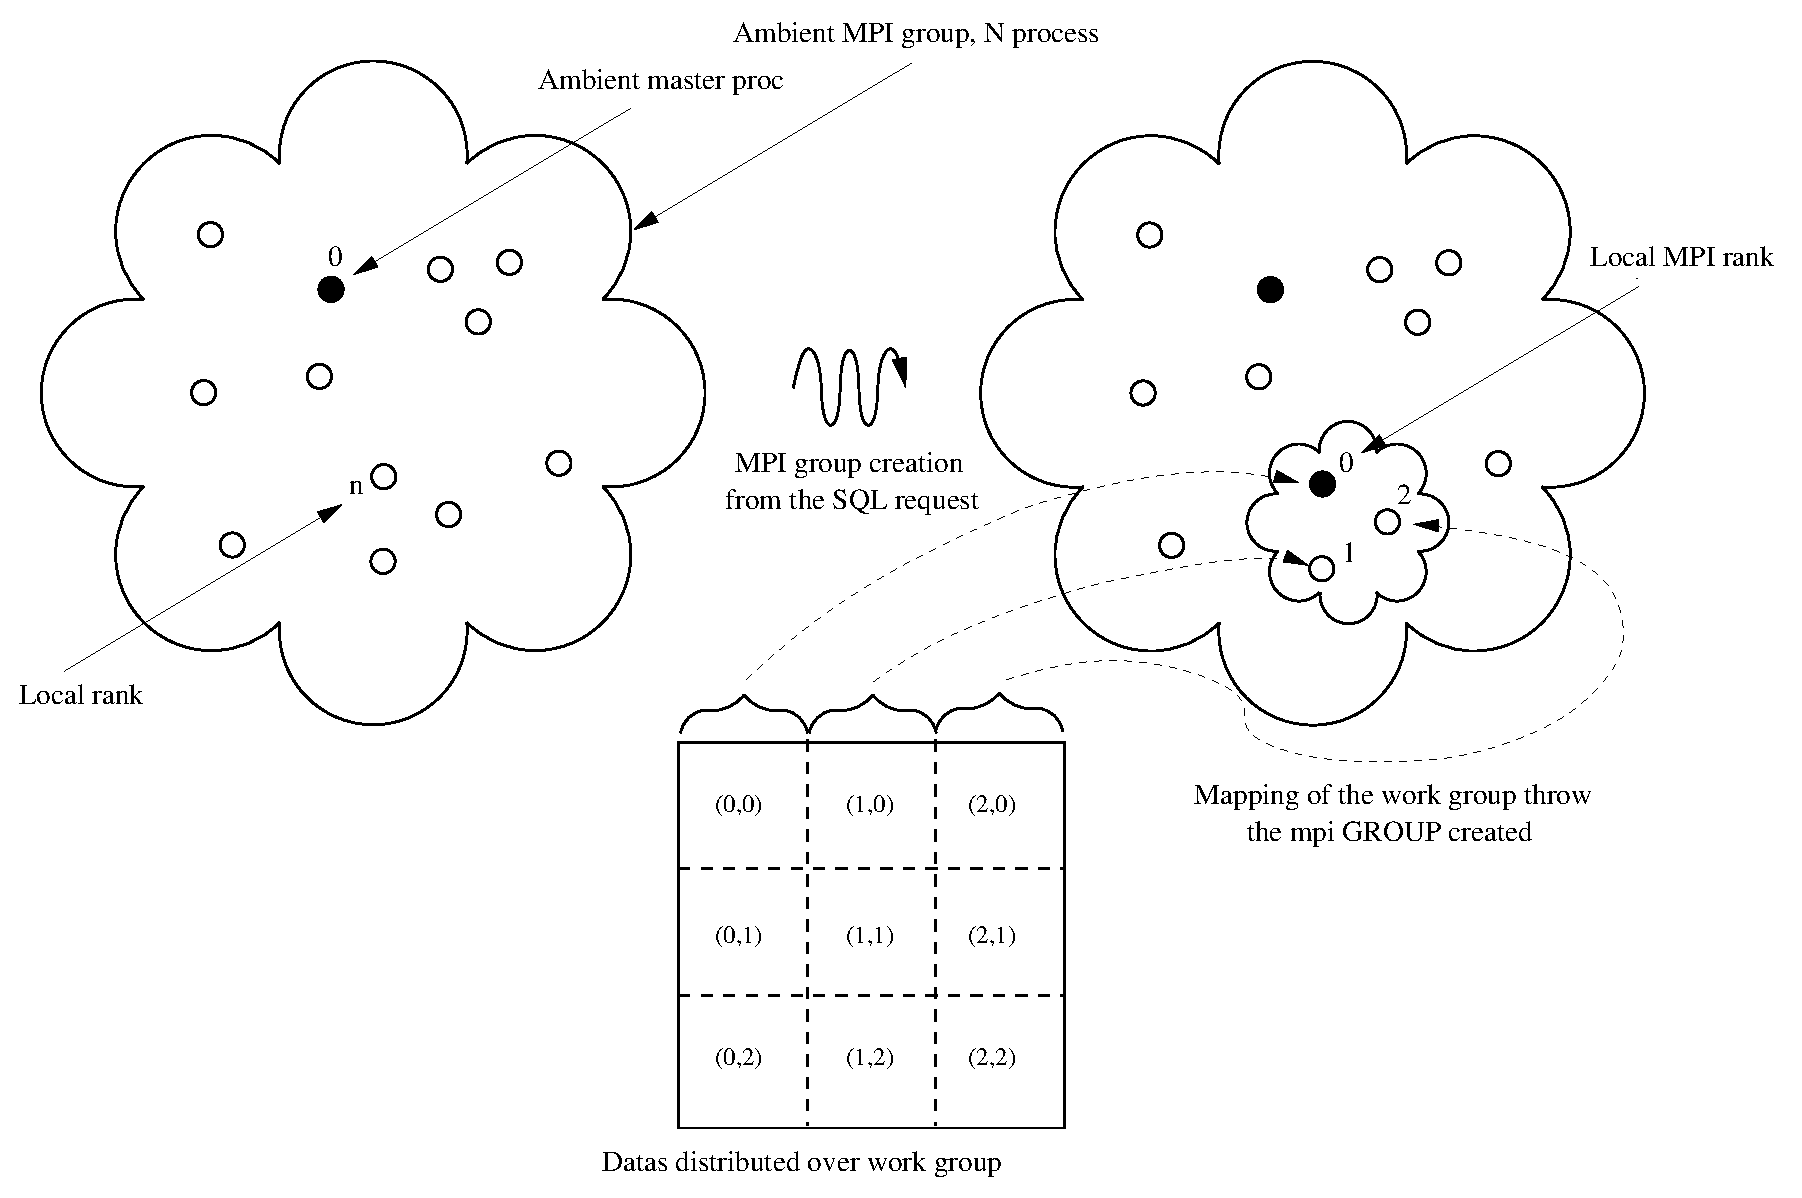
\includegraphics[scale=0.35]{FIGURES/MpiGroupData.eps} 
	\end{center}
          \caption[]{Creation of an MPI group using SQL request, with \hbox{\cloud \hspace{0.02cm}} representing an MPI group with its own communicator;  $\bullet$ represents the master 
          process inside the group whereas the $\circ$ are the associated slave processes inside the corresponding group. In this example the matrix is mapped block by block onto the processors using 1D column-cyclic distribution.}
          \label{MPIGROUP}
\end{figure}

After the SQL request section, the data is being mapped to the processes of the newly created MPI group in terms of work groups. Frequently the algorithm would be simply 1D or 2D block-cyclic distribution, the algorithm of which is described in table \ref{2DCYCLIC} (\cf Fig. \ref{MPIGROUP}). After the actual transfer, those processes will become the primary owners of their data in terms of storage and handling. With Ambient, every operation is associated with a pair of logistic and computational kernels - that is, there will be multiple SQL requests. In order to create new groups, processes from the parent group are being selected in queue fashion until all processes of the group have been selected. If more groups are required, the selection restarts from the beginning of the queue, thereby making those processes selected again simultaneous members of several groups. 

Every new group will have its own intra-communicator (allowing intra-group communication) as well as an inter-communicator (allowing communication between groups).

 \begin{table}[t] 
	\begin{center}
	 	\begin{tabular}{l l }
                           \hline 
                           \textbf{Assign workgroup}  Algorithm of the 1/2-D assign function  &    \\ \hline
                           \textbf{Require}        An new MPI group obtained by an SQL request  &  \\
                           \begin{tabular}{c l} 
                               \tiny{1:} &  Initialize $i$ in function of the new MPI rank  of the new group \\
                               \tiny{2:} &  Initialize $j$ in function of the new MPI rank  of the new group  $\vartriangleright$ Note:   \\
                                             &  the initialization of $i,j$ will fix   the distribution (1D or 2D) \\
                               \tiny{3:} &  \textbf{for} from $i$  to the number of the work group on $x$ \textbf{do} \\
                               \tiny{4:} &  \hspace{0.2 cm}  \textbf{for} from $j$  to the number of the work group on $y$ \textbf{do} \\
                               \tiny{5:} & \hspace{0.4 cm}    Assign the work group $(i,j)$ to the corresponding process\\
                               \tiny{6:} &   \hspace{0.2 cm}    \textbf{end for} \\
                               \tiny{7:} &  \textbf{end for} \\                               
                          \end{tabular} & \\ \hline
		 \end{tabular} 
		 \caption{Algorithm of the distribution of the work group into the new MPI group.   \label{2DCYCLIC}}
	\end{center}
\end{table} 

During execution, many groups will be created in practice, and data will have to be moved between groups.
To obtain better performance and to reduce the number of data transfers between groups, there are additional possible settings for the SQL request. For example, consider the previous illustration for the SQL request in case of the matrix addition operation ($ A \, +\!\!\!= B$).
If matrix $A$ has already been created and mapped on specific processors, the logistic kernel can create an MPI group as a subset or superset of the previous owner group (created in the previous operation), thereby avoiding superfluous data transfer. The concrete SQL request would be as follows:
 
\begin{eqnarray}  \label{SQL2}
         & & \texttt{scope\_select("\textit{N} from ambient as addition\_group }\\ 
         & & \texttt{	where master is 0 where breakdown contains" + get\_id(\textit{A})}), \nonumber
\end{eqnarray} 
The function \texttt{get\_id(\textit{A})} will get a tag  of \texttt{\textit{A}} to obtain its current binding.
 
%\begin{figure}[h]
%	\begin{center}
%			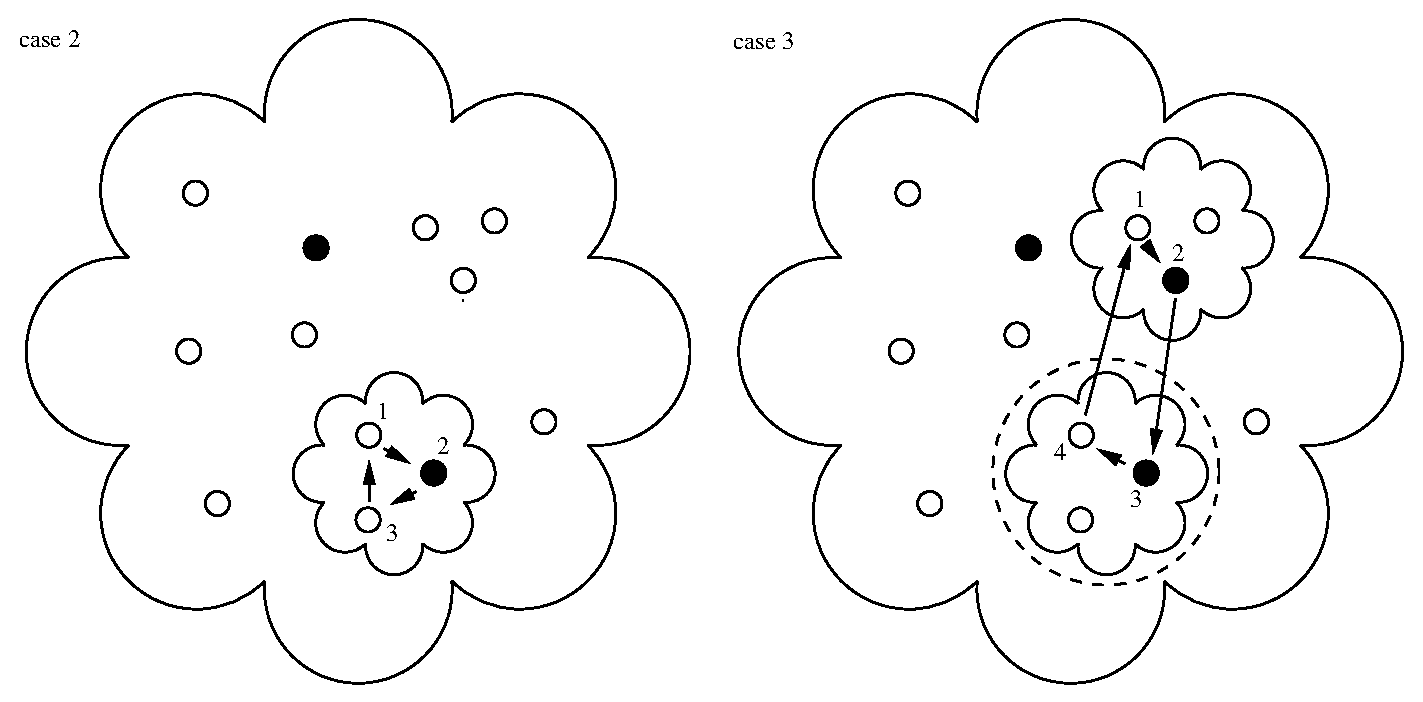
\includegraphics[scale=0.35]{FIGURES/ComGroup.eps} 
%	\end{center}
%          \caption{Data exchange inside the group.}
%          \label{COMGROUP}
%\end{figure}

%%%%%%%%%%%%%%%%%%%%%%%%%%%%% END SQL SECTION

%%%%%%%%%%%%%%%%%%%%%%%%%%%%% BEGINNING EXECUTION AND OPERATIONS SCHEDULING SECTION
\subsection{Execution model and Operations scheduling}
In a typical HPC application, the programming model imposes parallel execution of every function of the code, with data granularity imposing the details 
of the parallelization. In Ambient, we have made a scheduler that privileges a queue execution model where operations
are stacked up in a list first and are executed afterwards according to the respective logistic/computational kernel. This model is inspired by computer architecture design, i.e.
the queue data flow execution in a processor \cite{DENNIS-1974} (Alex: hell, no!).

Any HPC application can be decomposed into a set of functions performing numerical operations. Let's start from a basic example, where we want to perform the three following operations :

\begin{eqnarray} 
\text{Operation 1:} & & A + \!\! =  B, \label{3OPERATIONS}  \\
\text{Operation 2:} & & A \times \!\!= \lambda,   \nonumber  \\ 
\text{Operation 3:} & & C \times \!\!= D. \nonumber
\end{eqnarray}
with $A$, $B$, $C$ and $D$ being some matrices and $\lambda$ being some scalar.

Conventionally, each of these three operations would be executed in parallel, one after another. Transposing into Ambient's conception means associating each operation with a logistic and a computational kernel. Considering the example (\ref{3OPERATIONS}), one would invoke the following \texttt{push} function:

\begin{eqnarray}
     \texttt{push(Addition\_logistic, Addition\_computional, \textit{A}, \textit{B})},
\end{eqnarray} 

with the appropriate logistic and computational kernels \texttt{Addition\_logistic} and \texttt{Addition\_computational}  (c.f. table \ref{LKERNEL} and \ref{CKERNEL}), followed by the arguments \texttt{\textit{A}} and \texttt{\textit{B}}. This way, operations, such as those in (\ref{3OPERATIONS}), will stack up during execution of the application. At any time then, the operations on the stack would be available for the execution through the basic Ambient instruction

\begin{eqnarray}
      \texttt{playout()},
\end{eqnarray} 

although ideally this command would be invoked at the end, when all operations have been pushed onto the stack.
The \texttt{playout()} command triggers the Ambient engine to scan through the operation stack, identify the independent operations and mark dependencies. Next, a dedicated MPI packet manager\footnote{a tool managing the communication between processors.} (see section \ref{MPIABSTRACTION})  is added for each operation, and all logistic kernels for independent operations are executed. Next the computational kernels of these independent operations are executed. Following the completion of those, Ambient takes next chunk of independent operations (whose dependencies were just satisfied) and repeats the cycle transporting the necessary data to the new groups after the execution of logistic kernels is complete. In the case of data dependency, the data transfer is handled by the packet manager. When all computational kernels have been executed the stack is getting cleaned. The schematic overview of the stack execution is presented in Fig. \ref{EXECUTION} .

In overall, the Ambient employs single kernel multiple data parallelism model that is used over many process groups with different kernels and data.

\begin{figure}[h]
	\begin{center}
	      	        \psfrag{Operation 1}{\tiny{Operation 1}}
		        \psfrag{Operation 2}{\tiny{Operation 2}}
		        \psfrag{Operation 3}{\tiny{Operation 3}}
		        \psfrag{l/c kernel 1}{\tiny{l/c kernel 1}}
                           \psfrag{l/c kernel 2}{\tiny{l/c kernel 2}}
                           \psfrag{l/c kernel 3}{\tiny{l/c kernel 3}}
                           \psfrag{Ambient}{\tiny{Ambient}}
                           \psfrag{Schedule}{\tiny{Schedule}}
                           \psfrag{Dependency}{\tiny{Dependency}}
                           \psfrag{Time}{\tiny{Time}}
                           \psfrag{Evolution}{\tiny{evolution}}
                           \psfrag{Mapping and execution}{\tiny{Mapping and execution}}                          
                           \psfrag{Ambient execution}{\tiny{Ambient execution}}                          
                           \psfrag{Usual execution}{\tiny{Usual execution}}                          
	                  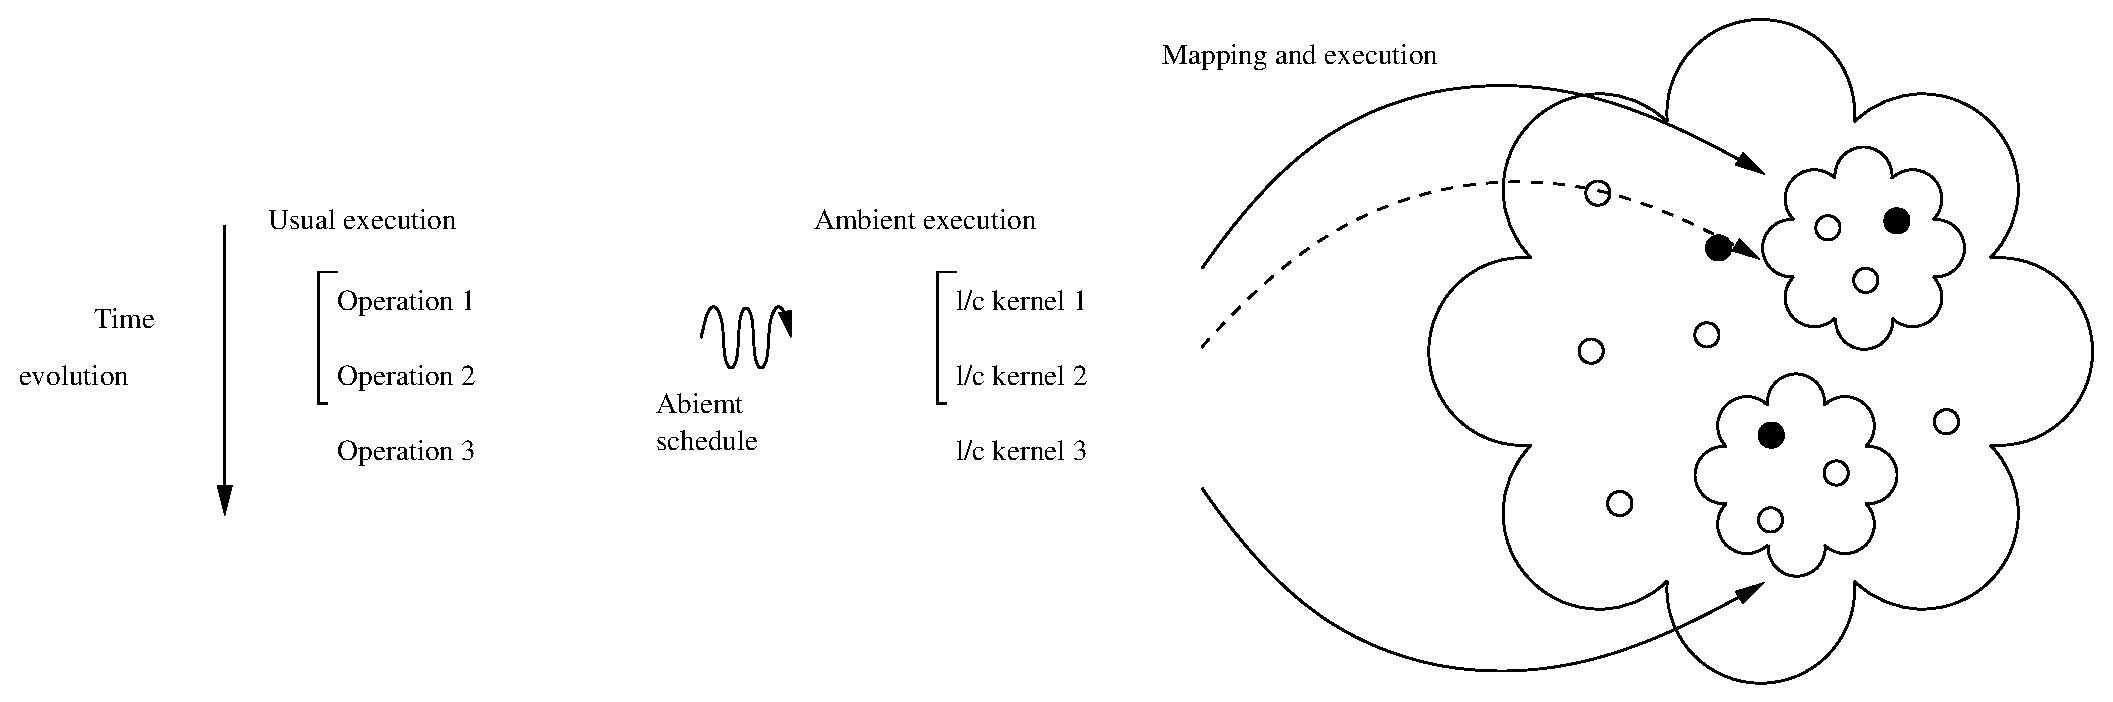
\includegraphics[scale=0.35]{FIGURES/execution.eps} 
	\end{center}
          \caption{Ambient scheduler's workflow model. On the classical approach (left) the operations will be executed in parallel step by step disregarding the dependencies (marked by the symbol \guillemotleft [\guillemotright \, in the schematic). In Ambient (right), operations will be associated to the logistic/computational kernel pair (abbreviate l/c), as operations 1 and 3  (l/c kernels 1 and 3) are independent - the execution of computational kernel will be performed simultaneously.  Due to the dependency between the kernel 1 and 2, the computational kernel of operation 2 (l/c kernel 2) will be executed later. It should be performed in a new MPI group but with an appropriate SQL request (\ref{SQL2}) in logistic kernel we can execute the computational kernel right in the place where the data currently is. }   \label{EXECUTION}
\end{figure}

Next, we generalize example \ref{3OPERATIONS} to deal with vectors of matrices. We assume conditional statements determining which matrices should be added and/or multipled (Table \ref{GRAPH}). First, from line 1 to 11, as a dry run, the application execution will determine which operations should be performed, 
pushing the required kernels on the top of the stack. When the \texttt{playout()} function is called in line 12, the engine will execute the stack. By resolving dependencies it will naturally create the directed acyclic graph of the application. 
\begin{table}[t] 
	\begin{center}
	 	\begin{tabular}{l l }
                           \hline 
                           Determination of the directed  acyclic graph   &    \\ \hline
                           \textbf{Require}    A class Matrix  that adheres Ambient architecture   &  \\  
                           and  vector of matrices  of size $n$, $A[n]$, $B[n]$, $C[n]$ and $D[n]$ & \\
                           \begin{tabular}{c l} 
                               \tiny{1:}   & \textbf{for} from $i$  to the size of the vector \textbf{do} \\
                               \tiny{2:}   & \hspace{0.2 cm} \textbf{for} from $j$  to the size of the vector \textbf{do} \\                               
                               \tiny{3:}   & \hspace{0.4 cm}  \textbf{if}  the conditions on $A[i]$ and  $B[j]$ are verified \textbf{do} \\                               
                               \tiny{4:}   & \hspace{0.8 cm}  $A[i]+ \!\! =B[j]$, $\vartriangleright$  push l/c kernel 1, \\
                               \tiny{5:}   & \hspace{0.4 cm} \textbf{end if} \\   
                               \tiny{6:}   & \hspace{0.4 cm} $A[i]\times \!\! =\lambda$,  $\vartriangleright$  push l/c kernel 2, \\                   
                               \tiny{7:}   & \hspace{0.4 cm} \textbf{if}  the conditions on $C[i]$ and  $D[j]$ are verified \textbf{do} \\                               
                               \tiny{8:}   & \hspace{0.8 cm} $C[i]\times \!\! =D[j]$,  $\vartriangleright$ push l/c kernel 3, \\
                               \tiny{9:}   & \hspace{0.4 cm}  \textbf{end if} \\       
                               \tiny{10:} & \hspace{0.2 cm}  \textbf{end do} \\   
                               \tiny{11:} & \textbf{end do} \\                                 
                               \tiny{12:} & \texttt{playout()} $\vartriangleright$  execute the stack \\
                               \tiny{13:} & $\vartriangleright$ Note:  $+\!\!=$ and $\times \!\! =$ operators have wrapper functions   \\
                                                & that push the good logistic and computational kernel. \\                               
                           \end{tabular}   &  \\ \hline
        	     \end{tabular}
	\end{center}
	\caption{Generalization of the example \ref{3OPERATIONS} with conditional statements. The cumulativeness of the stack and delayed manner of execution compromise the directed acyclic graph together. \label{GRAPH}}
\end{table} 

These examples demonstrate the strength of Ambient, allowing two levels of parallelization without any MPI hardcoding inside of the original code, with a great degree of flexibility and adaptability. 


%%%%%%%%%%%%%%%%%%%%%%%%%%%%% END EXECUTION AND OPERATIONS SCHEDULING SECTION


%%%%%%%%%%%%%%%%%%%%%%%%%%%%% BEGIN PACKET MANAGER 
\subsection{Packet manager and MPI abstraction} \label{MPIABSTRACTION}
In standard HPC applications, data may have to be prepared for exchange over the network, particularly if the data is of more than one type; in the latter case,
an MPI structure is set up, to which the data is then copied, and then this structure is sent via network. These preliminary conversions can cut into
performance. In Ambient, the data layout inside each work group necessitates additional metadata to coordinate the execution of logistic and 
computational kernels, particularly the latter has to perform a remote access. Thus, the block of data associated with a workgroup exists only in the form that includes meta-data 
in contiguous memory layout manner. We use this ensemble \guillemotleft block of data + metadata\guillemotright \, directly as a network packet based on top of MPI derived datatypes. 
Thereby, work groups can move around without additional overhead on copying and any other composure. 
To assure proper execution of the framework, several additional type of packets are available: control packet, layout packet and data-block packet that derive from one standard packet type. 

During the computational kernel execution, one can access any required remote data, such as a block of matrix $A$, by use of the Ambient modificator  \texttt{current(\textit{A})(i,j)}
(ref. \ref{CURRENT}), where \textit{A} has to be a matrix or other object that adheres Ambient's architecture (\cite{ABSTRACTPARADATATYPE}), the indices $i$ and $j$ are the coordinates of the work group (Fig. \ref{MPIGROUP}). 
There are three possibilities of resulting communication while a process issues data via modificators inside computational kernel:

\begin{enumerate}
\item \textit{The work group is already in the memory of the process.} The access is direct.
\item \textit{The work group is in the memory space of the present MPI-group (previously created by the associated logistic kernel).} 
The process requiring this data sends a query (a specific type of packet) to the master process of its MPI group.
The master process, which knows which slave process of its' group holds the required work group, sends a new request to
that process, which in turn sends the requested workgroup to the requesting process. 
\item \textit{The work group is held inside another MPI-group.} As previously, the process which executes the computational kernel sends a query to the master process of its MPI group,
which in turn sends a request to the master process of the MPI group within which the data is held. That master process then sends a message to the actual owner process,
which finally sends the data to the initially requesting process.
\end{enumerate}
Case (2) and (3) are illustrated in Fig. \ref{MPIEXCHANGE}.
\begin{figure}[h]
	\begin{center}
	    \psfrag{case 2}{\tiny case 2}
	    \psfrag{case 3}{\tiny case 3}
             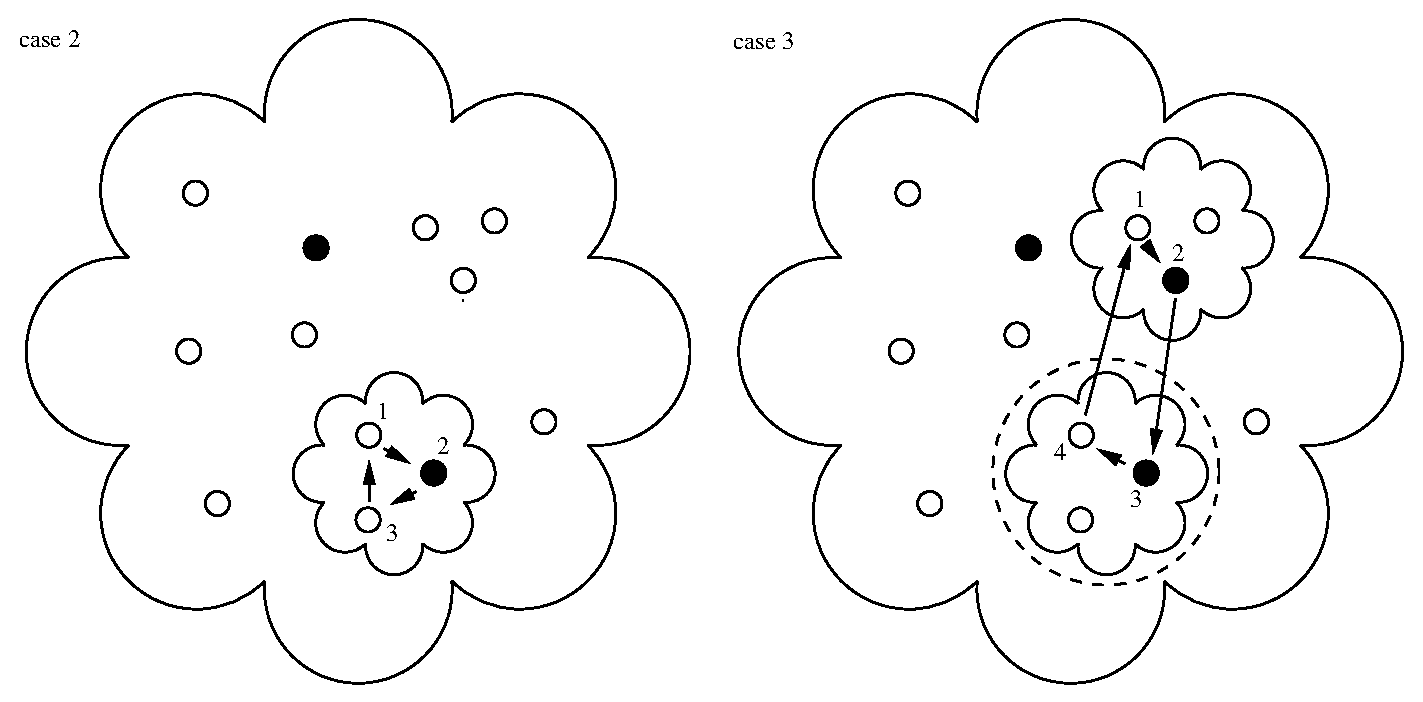
\includegraphics[scale=0.35]{FIGURES/ComGroup.eps} 
	\end{center}
          \caption{On the left: communications inside the same group. On the right: communications between two MPI-groups. The dashed circle indicates the group holding the requested data.
          In both cases, the master processes have a key role in distributing information for the exchange. Each arrow marks a request, the sequence of requests is enumerated.}  \label{MPIEXCHANGE}
\end{figure}

Clearly, smooth execution of any communication pattern arising from the great number of possible data dependencies
is key to a good performance of the Ambient approach. The resolution of communication patters also falls under the purview
of the packet manager, as it manages both intra- and inter-group communication. Each MPI-group has its own singleton packet manager.

To reach the best performance in HPC, bottlenecks arising from synchronization operations should be avoided  \cite{EXASCALE-2010}.
Thus, MPI asynchronous communication is privileged in Ambient (\texttt{mpi\_isend} and \texttt{mpi\_irecv}). As we avoid synchronization 
instructions, the process repeatedly checks for the availability of the incoming data in an infinite loop, until actually receiving the
data.

For the packet manager to be adaptable to any communication pattern, it employs the delegate mechanism and a finite state machine (FSM).

\begin{table}[b] 
	\begin{center}
	 	\begin{tabular}{l l }
                           \hline 
                           Algorithm of the packet manager   &    \\ \hline
                           \textbf{Require}  a MPI process requires a block of data &  \\                           
                            \begin{tabular}{c l}                                
                               \tiny{1:}   & \textbf{for}  ;;  \textbf{do} $\vartriangleright$  infinite loop \\
                               \tiny{2:}   & \hspace{0.2 cm}  \texttt{Delegate()}  $\vartriangleright$ check if packet has been \\
                                                & received, and re-send if needed \\
                               \tiny{3:}   & \hspace{0.2 cm}  FSM $\vartriangleright$ break the loop, \\
                                               & if all packets have arrived at destination. \\
                               \tiny{4:}   & \textbf{end do} \\
                           \end{tabular}   &  \\ \hline
        	     \end{tabular}
	\end{center}
	\caption{Description of the packet manager}
\end{table} 



%\begin{figure}[h]
%	\begin{center}
%	    \psfrag{1}{\tiny \hspace{-0.1 cm}  1}
%	    \psfrag{2}{\tiny \hspace{-0.1 cm}  2}
%	    \psfrag{Loose}{\tiny \hspace{-0.2 cm}   Loose}
%	    \psfrag{Closure}{\tiny \hspace{-0.2 cm}  Closure}
%	    \psfrag{Open}{\tiny \hspace{-0.4 cm}  Opening}
%          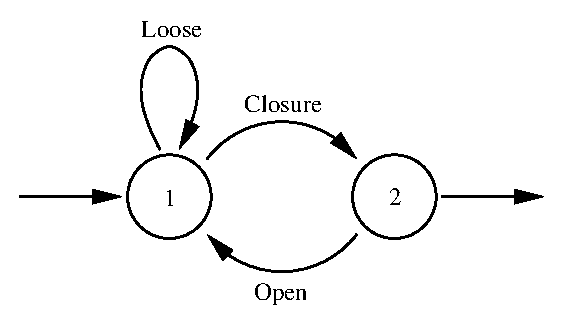
\includegraphics[scale=0.45]{FIGURES/FSM.eps} 
%	\end{center}
%          \caption{Schematic of the finite sate machine for the closing procedure. The states 1 and 2 correspond to open or close.
%           The transitions are loose, closure or opening, they  depend of the situation of all packets (if they all reach theirs targets or not),
%                          the loose transition means the packet has not been received, thus we iterate one more time on the infinite loop.}  \label{FSM}
%\end{figure}

The delegate mechanism serves its design goal - to execute handlers of components listening for the packets arrival, such as layout tables.
This delegate object inside the packet manager is tied to a list of functions, such as layout forwarding, 
data block forwarding and control information handlers. As the packet manager checks for completion of the local send process, the finite state machine
checks the send completion state of the other MPI processes (whether they have sent all their packets or not). If all the packets have been sent, the FSM breaks the infinite loop.


%%%%%%%%%%%%%%%%%%%%%%%%%%%%% END PACKET MANAGER 

%%%%%%%%%%%%%%%%%%%%%%%%%%%%% BEGIN ABSTRACT PARALLEL DATATYPES 
\subsection{Abstract parallel datatypes} \label{ABSTRACTPARADATATYPE}

To assure that Ambient has the largest possible scope, we designed the framework on the data structures and not on a specific problem. Thus, we enlarge the utilization of the framework
to encompass various applied computing fields. The connection  between Ambient and the \guillemotleft outside world \guillemotright  \, is done by an intermediate class that assures the
adherance of class to Ambient's architecture.

For linear algebra, we designed a matrix class which contains the usual data members for describing the object (number of rows, number of columns, \dots) and methods for linear
algebra operations (associated with logistic and computational kernels). This matrix class derives from another one which ensures the adherence to Ambient's architecture.

%%%%%%%%%%%%%%%%%%%%%%%%%%%%% END ABSTRACT PARALLEL DATATYPES 


%%%%%%%%%%%%%%%%%%%%%%%%%%%%% BEGIN VALIDATION
\subsection{Validation}
As a validation test, we code a new implementation of PDGEMM using the Ambient framework, and compare to the ScaLAPACK version of PDGEMM (MKL-Version).
The algorithm of our implementation is based on the classical method [CITATION NEEDED] using a column order distribution for the matrices (\cf table \ref{AMBIENTDGEMM} 
for the modification due to Ambient). The main advantage in our implementation is the required amount of coding, which is limited to seven lines.

----------------------------------------------------------------------------------------------------- \\
TO DO: EXPLAIN THE ADVANTAGE AGAINST   SCALAPACK \\
IN TERM OF NETWORK, DATA EXCHANGE \\
----------------------------------------------------------------------------------------------------- \\

We compare the Ambient results with the ScaLAPACK implementation. As related in section \ref{CUDAIDEOLOGYSECTION}, Ambient is compatible with ScaLAPACK,
despite the difference in memory layout. In Ambient, each work group is principally independent from any other, even if they belong to the same process, while in ScaLAPACK
blocks are grouped by process s.t. a memory-contiguous object is obtained. Therefore, calling a ScaLAPACK solver from Ambient must entail rearrangement of appropriate
work groups into a contiguous blocks, and thus a certain overhead. Due to Ambients flexibility in handling and grouping data, from a programming perspective this task
is simple to accomplish however. 

 \begin{table}[t] 
	\begin{center}
	 	\begin{tabular}{l l }
                           \hline 
                           \textbf{ Algorithm:}  pDGEMM using Ambient  &    \\ \hline
                           \textbf{Require}                 A pinned computational kernel  &  \\
                           \begin{tabular}{c l} 
                                 \tiny{1:} &  Get the cartesian coordinate $i,j$ of the work group \\ 
                                 \tiny{2:} &  Refer  the  work group$(i,j)$  of B into $B_{ref}$ \\
                                 \tiny{3:} &  \textbf{for} from $k(0)$  to the max number of rows \textbf{do} \\
                                 \tiny{4:} &  \hspace{0.2 cm} Refer  the  work group$(k,j)$  of A into $A_{ref}$ \\    
                                 \tiny{5:} &  \hspace{0.2 cm}  reduction of the blocks $(k,i)$ into $C_{ref}$ , $\vartriangleright$  The reduction, \\
                                                & \hspace{0.2 cm}  is done by a proxy pattern \\
                                 \tiny{6:} &  \hspace{0.2 cm}  classical DGEMM($A_{ref}$, $B_{ref}$, $C_{ref}$)\\
                                 \tiny{7:} &  \textbf{end do} \\    
                             \end{tabular} & \\ \hline
		 \end{tabular} 
		 \caption{Algorithm of the pDGEMM using Ambient framework. We remember a proxy pattern is an interface the something else (object in memory). There, it allows the reduction between the independent workgroups.   \label{AMBIENTDGEMM}}
	\end{center}
\end{table} 

The validation test consists of multiplying matrices and saving the results into an output matrix, $C = A \times B$,
where we further compare between the output of the Ambient computational kernel and the ScaLAPACK PDGEMM solver.
Using the C++ language, the operations $\times$ and $=$ have been overloaded appropriately, now containing the "pushing" of the required logistic and computational kernels.
Afterwards, results are compared element by element using the test  \cite{Dongarra:1990:SLB:77626.79170}  $\left \lvert C^S_{ij} - C^A_{ij} \right \rvert/\left \lvert  \epsilon C^S_{ij} \right \rvert  < n$,
where  the precision factor $\epsilon$  is the \texttt{double} precision $10^{-16}$, indices  $S$ and $A$ represent the ScaLAPACK and the Ambient version, and $n=16$, the exponent of numerical precision. 

For the test, the size of work groups has been fixed to $128 \times 128$, and the square matrices $A$, $B$ range from 256 up to 8196 in size (step size of 128). The numbers of MPI-Process varied from 2 to 8.
Matrices were filled upusing a pseudo random number generator  \texttt{drand48()}\footnote{This function returns 
pseudo-random numbers non-negative, double-precision,  uniformly distributed over the interval $[0, 1]$ using a linear congruential algorithm and 
48-bit integer arithmetic. }  from \texttt{stdlib}.  
%%%%%%%%%%%%%%%%%%%%%%%%%%%%% END VALIDATION



%%%%%%%%%%%%%%%%%%%%%%%%%%%%% END DESCRIPTION OF THE FRAMEWORK

\section{Results and discussions}
\subsection{First benchmark case}
[STARTED REWRITING THIS; BUT NOT FINISHED]
The first benchmark consists of evaluating the performance of our parallel matrix multiplication relative to the iScaLAPACK-MKL mplementation. Both solvers are included as computational kernels
in Ambient.  The initial condition are the same than the validation test. As the validation test, the matrices size vary from 256 up to 8196 by step of (128 elements). A 1-D cyclic  column distribution is
used for both algorithm. As both kernels are included inside the framework additional workload should take into account and for the ScaLAPACK pDGEMM, we reorganize data to fit the ScaLAPACK
representation. The benchmarks  were performed on AMD Opteron  Magny-Cours) CPUs at 2.1 GHz on the Swiss National Supercomputing Centre facilities. The performance is reported in [GFlops], it is simply
calculated by :

\begin{eqnarray}
P  = \frac{2n^i}{t},
\end{eqnarray}
where $n$ is the size of the square-matrix,  $t$ the full time of calculation and $i$ is equal to 3 for the classical matrix multiplication algorithm.

\begin{figure}
% GNUPLOT: LaTeX picture with Postscript
\begingroup
  \makeatletter
  \providecommand\color[2][]{%
    \GenericError{(gnuplot) \space\space\space\@spaces}{%
      Package color not loaded in conjunction with
      terminal option `colourtext'%
    }{See the gnuplot documentation for explanation.%
    }{Either use 'blacktext' in gnuplot or load the package
      color.sty in LaTeX.}%
    \renewcommand\color[2][]{}%
  }%
  \providecommand\includegraphics[2][]{%
    \GenericError{(gnuplot) \space\space\space\@spaces}{%
      Package graphicx or graphics not loaded%
    }{See the gnuplot documentation for explanation.%
    }{The gnuplot epslatex terminal needs graphicx.sty or graphics.sty.}%
    \renewcommand\includegraphics[2][]{}%
  }%
  \providecommand\rotatebox[2]{#2}%
  \@ifundefined{ifGPcolor}{%
    \newif\ifGPcolor
    \GPcolorfalse
  }{}%
  \@ifundefined{ifGPblacktext}{%
    \newif\ifGPblacktext
    \GPblacktexttrue
  }{}%
  % define a \g@addto@macro without @ in the name:
  \let\gplgaddtomacro\g@addto@macro
  % define empty templates for all commands taking text:
  \gdef\gplbacktext{}%
  \gdef\gplfronttext{}%
  \makeatother
  \ifGPblacktext
    % no textcolor at all
    \def\colorrgb#1{}%
    \def\colorgray#1{}%
  \else
    % gray or color?
    \ifGPcolor
      \def\colorrgb#1{\color[rgb]{#1}}%
      \def\colorgray#1{\color[gray]{#1}}%
      \expandafter\def\csname LTw\endcsname{\color{white}}%
      \expandafter\def\csname LTb\endcsname{\color{black}}%
      \expandafter\def\csname LTa\endcsname{\color{black}}%
      \expandafter\def\csname LT0\endcsname{\color[rgb]{1,0,0}}%
      \expandafter\def\csname LT1\endcsname{\color[rgb]{0,1,0}}%
      \expandafter\def\csname LT2\endcsname{\color[rgb]{0,0,1}}%
      \expandafter\def\csname LT3\endcsname{\color[rgb]{1,0,1}}%
      \expandafter\def\csname LT4\endcsname{\color[rgb]{0,1,1}}%
      \expandafter\def\csname LT5\endcsname{\color[rgb]{1,1,0}}%
      \expandafter\def\csname LT6\endcsname{\color[rgb]{0,0,0}}%
      \expandafter\def\csname LT7\endcsname{\color[rgb]{1,0.3,0}}%
      \expandafter\def\csname LT8\endcsname{\color[rgb]{0.5,0.5,0.5}}%
    \else
      % gray
      \def\colorrgb#1{\color{black}}%
      \def\colorgray#1{\color[gray]{#1}}%
      \expandafter\def\csname LTw\endcsname{\color{white}}%
      \expandafter\def\csname LTb\endcsname{\color{black}}%
      \expandafter\def\csname LTa\endcsname{\color{black}}%
      \expandafter\def\csname LT0\endcsname{\color{black}}%
      \expandafter\def\csname LT1\endcsname{\color{black}}%
      \expandafter\def\csname LT2\endcsname{\color{black}}%
      \expandafter\def\csname LT3\endcsname{\color{black}}%
      \expandafter\def\csname LT4\endcsname{\color{black}}%
      \expandafter\def\csname LT5\endcsname{\color{black}}%
      \expandafter\def\csname LT6\endcsname{\color{black}}%
      \expandafter\def\csname LT7\endcsname{\color{black}}%
      \expandafter\def\csname LT8\endcsname{\color{black}}%
    \fi
  \fi
  \setlength{\unitlength}{0.0500bp}%
  \begin{picture}(7200.00,4536.00)%
    \gplgaddtomacro\gplbacktext{%
      \csname LTb\endcsname%
      \put(814,704){\makebox(0,0)[r]{\strut{} 0}}%
      \put(814,1299){\makebox(0,0)[r]{\strut{} 5}}%
      \put(814,1893){\makebox(0,0)[r]{\strut{} 10}}%
      \put(814,2488){\makebox(0,0)[r]{\strut{} 15}}%
      \put(814,3082){\makebox(0,0)[r]{\strut{} 20}}%
      \put(814,3677){\makebox(0,0)[r]{\strut{} 25}}%
      \put(814,4271){\makebox(0,0)[r]{\strut{} 30}}%
      \put(1513,484){\makebox(0,0){\strut{} 1024}}%
      \put(2269,484){\makebox(0,0){\strut{} 2048}}%
      \put(3024,484){\makebox(0,0){\strut{} 3072}}%
      \put(3780,484){\makebox(0,0){\strut{} 4096}}%
      \put(4536,484){\makebox(0,0){\strut{} 5120}}%
      \put(5292,484){\makebox(0,0){\strut{} 6144}}%
      \put(6047,484){\makebox(0,0){\strut{} 7168}}%
      \put(6803,484){\makebox(0,0){\strut{} 8192}}%
      \put(176,2487){\rotatebox{-270}{\makebox(0,0){\strut{}GFlops}}}%
      \put(3874,154){\makebox(0,0){\strut{}Matrix size}}%
    }%
    \gplgaddtomacro\gplfronttext{%
      \csname LTb\endcsname%
      \put(5816,4098){\makebox(0,0)[r]{\strut{}Peak}}%
      \csname LTb\endcsname%
      \put(5816,3878){\makebox(0,0)[r]{\strut{}pDGEMM ScaLAPACK}}%
      \csname LTb\endcsname%
      \put(5816,3658){\makebox(0,0)[r]{\strut{}pDGEMM Ambient}}%
    }%
    \gplbacktext
    \put(0,0){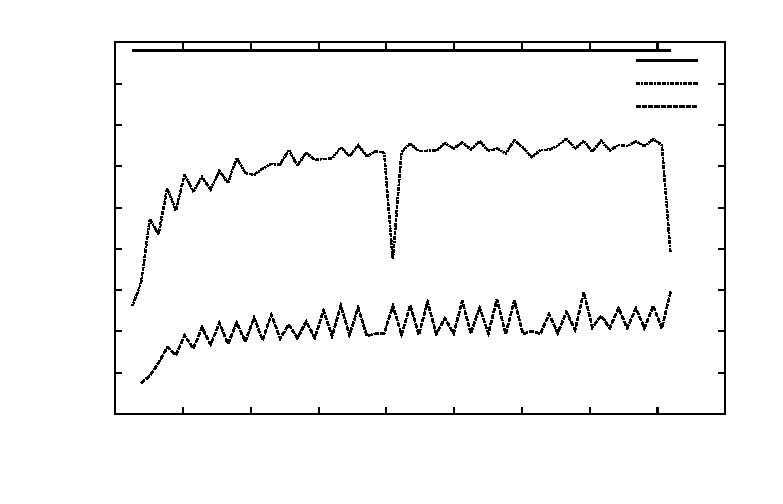
\includegraphics{SinglePGEMM}}%
    \gplfronttext
  \end{picture}%
\endgroup

\caption{Performances of PDGEMM using ScaLAPACK }
\end{figure}

\subsection{Second benchmark case}
This benchmarks consists to evaluate the performance of the scheduler, especially the repartition of several operation all over the cluster. 

\begin{figure}
% GNUPLOT: LaTeX picture with Postscript
\begingroup
  \makeatletter
  \providecommand\color[2][]{%
    \GenericError{(gnuplot) \space\space\space\@spaces}{%
      Package color not loaded in conjunction with
      terminal option `colourtext'%
    }{See the gnuplot documentation for explanation.%
    }{Either use 'blacktext' in gnuplot or load the package
      color.sty in LaTeX.}%
    \renewcommand\color[2][]{}%
  }%
  \providecommand\includegraphics[2][]{%
    \GenericError{(gnuplot) \space\space\space\@spaces}{%
      Package graphicx or graphics not loaded%
    }{See the gnuplot documentation for explanation.%
    }{The gnuplot epslatex terminal needs graphicx.sty or graphics.sty.}%
    \renewcommand\includegraphics[2][]{}%
  }%
  \providecommand\rotatebox[2]{#2}%
  \@ifundefined{ifGPcolor}{%
    \newif\ifGPcolor
    \GPcolortrue
  }{}%
  \@ifundefined{ifGPblacktext}{%
    \newif\ifGPblacktext
    \GPblacktexttrue
  }{}%
  % define a \g@addto@macro without @ in the name:
  \let\gplgaddtomacro\g@addto@macro
  % define empty templates for all commands taking text:
  \gdef\gplbacktext{}%
  \gdef\gplfronttext{}%
  \makeatother
  \ifGPblacktext
    % no textcolor at all
    \def\colorrgb#1{}%
    \def\colorgray#1{}%
  \else
    % gray or color?
    \ifGPcolor
      \def\colorrgb#1{\color[rgb]{#1}}%
      \def\colorgray#1{\color[gray]{#1}}%
      \expandafter\def\csname LTw\endcsname{\color{white}}%
      \expandafter\def\csname LTb\endcsname{\color{black}}%
      \expandafter\def\csname LTa\endcsname{\color{black}}%
      \expandafter\def\csname LT0\endcsname{\color[rgb]{1,0,0}}%
      \expandafter\def\csname LT1\endcsname{\color[rgb]{0,1,0}}%
      \expandafter\def\csname LT2\endcsname{\color[rgb]{0,0,1}}%
      \expandafter\def\csname LT3\endcsname{\color[rgb]{1,0,1}}%
      \expandafter\def\csname LT4\endcsname{\color[rgb]{0,1,1}}%
      \expandafter\def\csname LT5\endcsname{\color[rgb]{1,1,0}}%
      \expandafter\def\csname LT6\endcsname{\color[rgb]{0,0,0}}%
      \expandafter\def\csname LT7\endcsname{\color[rgb]{1,0.3,0}}%
      \expandafter\def\csname LT8\endcsname{\color[rgb]{0.5,0.5,0.5}}%
    \else
      % gray
      \def\colorrgb#1{\color{black}}%
      \def\colorgray#1{\color[gray]{#1}}%
      \expandafter\def\csname LTw\endcsname{\color{white}}%
      \expandafter\def\csname LTb\endcsname{\color{black}}%
      \expandafter\def\csname LTa\endcsname{\color{black}}%
      \expandafter\def\csname LT0\endcsname{\color{black}}%
      \expandafter\def\csname LT1\endcsname{\color{black}}%
      \expandafter\def\csname LT2\endcsname{\color{black}}%
      \expandafter\def\csname LT3\endcsname{\color{black}}%
      \expandafter\def\csname LT4\endcsname{\color{black}}%
      \expandafter\def\csname LT5\endcsname{\color{black}}%
      \expandafter\def\csname LT6\endcsname{\color{black}}%
      \expandafter\def\csname LT7\endcsname{\color{black}}%
      \expandafter\def\csname LT8\endcsname{\color{black}}%
    \fi
  \fi
  \setlength{\unitlength}{0.0500bp}%
  \begin{picture}(7200.00,4536.00)%
    \gplgaddtomacro\gplbacktext{%
      \csname LTb\endcsname%
      \put(946,704){\makebox(0,0)[r]{\strut{} 0}}%
      \put(946,1417){\makebox(0,0)[r]{\strut{} 20}}%
      \put(946,2131){\makebox(0,0)[r]{\strut{} 40}}%
      \put(946,2844){\makebox(0,0)[r]{\strut{} 60}}%
      \put(946,3558){\makebox(0,0)[r]{\strut{} 80}}%
      \put(946,4271){\makebox(0,0)[r]{\strut{} 100}}%
      \put(1078,484){\makebox(0,0){\strut{} 0}}%
      \put(2223,484){\makebox(0,0){\strut{} 10}}%
      \put(3368,484){\makebox(0,0){\strut{} 20}}%
      \put(4513,484){\makebox(0,0){\strut{} 30}}%
      \put(5658,484){\makebox(0,0){\strut{} 40}}%
      \put(6803,484){\makebox(0,0){\strut{} 50}}%
      \put(176,2487){\rotatebox{-270}{\makebox(0,0){\strut{}Absolute difference \%}}}%
      \put(3940,154){\makebox(0,0){\strut{}Number of product of matrices}}%
    }%
    \gplgaddtomacro\gplfronttext{%
      \csname LTb\endcsname%
      \put(5816,1317){\makebox(0,0)[r]{\strut{}$M = 512$}}%
      \csname LTb\endcsname%
      \put(5816,1097){\makebox(0,0)[r]{\strut{}$M = 1024$}}%
      \csname LTb\endcsname%
      \put(5816,877){\makebox(0,0)[r]{\strut{}$M = 2048$}}%
    }%
    \gplbacktext
    \put(0,0){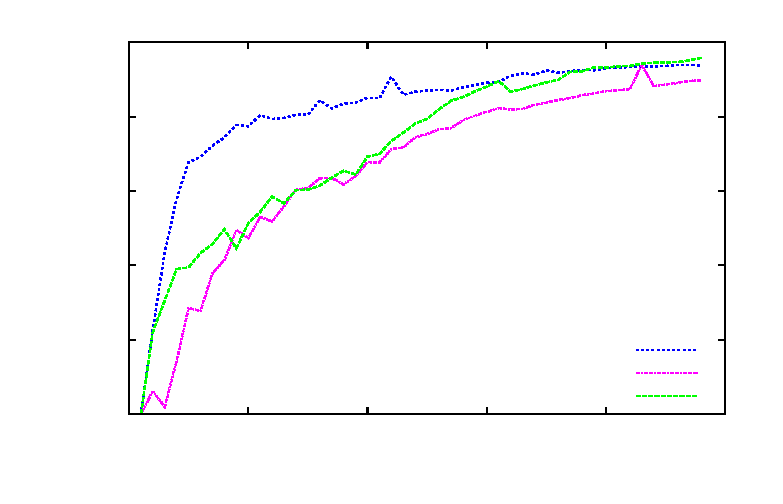
\includegraphics{VectorPGEMM}}%
    \gplfronttext
  \end{picture}%
\endgroup

\caption{Performances of a vector of PDGEMM using ScaLAPACK}
\end{figure}


\subsection{Third benchmark case}





\section{Conclusions}

%%%%%%%%%%%%%%%%%%%%%%%%%%%%% BEGIN THANK 
\thanks{The authors are grateful to W. Sawyer and G. Fourestey from the CSCS staff and V. Rezzonico from EPFL.} 
%%%%%%%%%%%%%%%%%%%%%%%%%%%%% END THANK 



%%%%%%%%%%%%%%%%%%%%%%%%%%%%% BEGIN BIBLIO
\bibliographystyle{abbrv}
\bibliography{biblio}
%%%%%%%%%%%%%%%%%%%%%%%%%%%%% END BIBLIOr



\end{document}  
